\documentclass[11pt]{book}
\usepackage{pdfpages}
\usepackage{fancyhdr}
\usepackage{multicol}
\usepackage[utf8]{inputenc}
\usepackage[top=48pt,headheight=18pt,headsep=12pt,bottom=48pt,inner=48pt,outer=48pt]{geometry}

\begin{document}

\pagestyle{fancy}

\fancyhf{}

\fancyhead[LE,RO]{\thepage}
\fancyhead[C]{   \leftmark }
\fancyfoot[C]{
Ganassi Embellishments \textit{Regola Prima}
}

\fancypagestyle{FooBar}{%
  \fancyhead{}
  \fancyhead[LE,RO]{\thepage}
}
\fancypagestyle{NoHead}{%
  \fancyhead{}
  
}

\renewcommand{\headrulewidth}{0pt}
\renewcommand{\footrulewidth}{0pt}
\renewcommand{\chaptermark}[1]{\markboth{\MakeUppercase{#1}}{}}

\setlength{\parindent}{0pt}
\setlength{\parskip}{11pt plus 2pt minus 4pt}

\begin{titlepage}
    \centering
    \vspace*{2.5cm}
    {\scshape\Large An aide to practicing the embellishments in Sylvestro Ganassi's\\ 
    \em{Opera Intitulata Fontegara}. \par}
    \vspace{1cm}
    {\scshape\Huge Ganassi Embellishments} \\
    {\scshape \Huge \textit{Regola Prima} \par}
    \vspace{1cm}
    {\scshape\normalsize Monique Rio, June 5, 2017 \par}
    \vspace{2cm}
    \vfill
    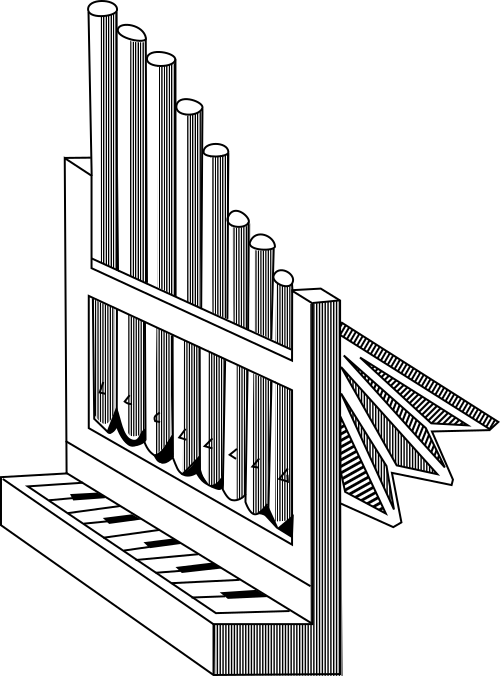
\includegraphics[scale=.5]{stcpress.png}\\
    {\large St. Cecilia Press}
\end{titlepage}

\clearpage
\thispagestyle{NoHead}
\section*{Table of Contents}


\noindent
Preface \dotfill i\\
\\
Unison \dotfill \pageref{unison} \\
Ascending Second \dotfill \pageref{ascending_second} \\
Descending Second \dotfill \pageref{descending_second} \\
Ascending Third \dotfill \pageref{ascending_third} \\
Descending Third \dotfill \pageref{descending_third} \\
Ascending Fourth \dotfill \pageref{ascending_fourth} \\
Descending Fourth \dotfill \pageref{descending_fourth} \\
Ascending Fifth \dotfill \pageref{ascending_fifth} \\
Descending Fifth \dotfill \pageref{descending_fifth} \\
Cadences \dotfill \pageref{cadences} 
%\begin{figure}[b!]
%\begin{center}
%\includegraphics[height=3in]{capriole.pdf}
%\end{center}
%\end{figure}

\pagenumbering{roman}
\setcounter{page}{1}
\section*{Preface}
This book contains the \textit{Regola Prima} embellishment examples from Sylvestro Ganassi's 1535 \textit{Opera Intitulata Fontegara}.	The original book is written for recorder players, but the embellishments work on any instrument. The embellishment examples have been transposed into 7 positions on the staff to ease practicing over all notes and intervals. No clef is notated; use whichever works for your instrument. No key is notated; use whatever key you want. Likewise, you should apply musica ficta as necessary. 

In transposing the examples, I've set the ambitus to be 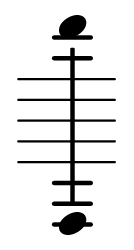
\includegraphics[height=3em]{snippit.png}. Any examples that exceed this ambitus have been removed for that transposition. 


I recommend playing the unornamented interval or cadence before playing each embellishment. This way the embellishment is linked to the unornamented line and will be more easily recognized by your ear and your muscle memory. 

Once you have an embellishment in your fingers, apply it to some music. Dance tunes are particularly good for ornamenting as are many 16th century melodies.

I hope you find this book useful in bringing 16th century ornamentation into your playing. 
\begin{flushright}
\textsc{Monique Rio}
\end{flushright}

\clearpage
\pagenumbering{arabic}
\setcounter{page}{1}
%\chapter*{Unison}
\chaptermark{Unison}\thispagestyle{FooBar}

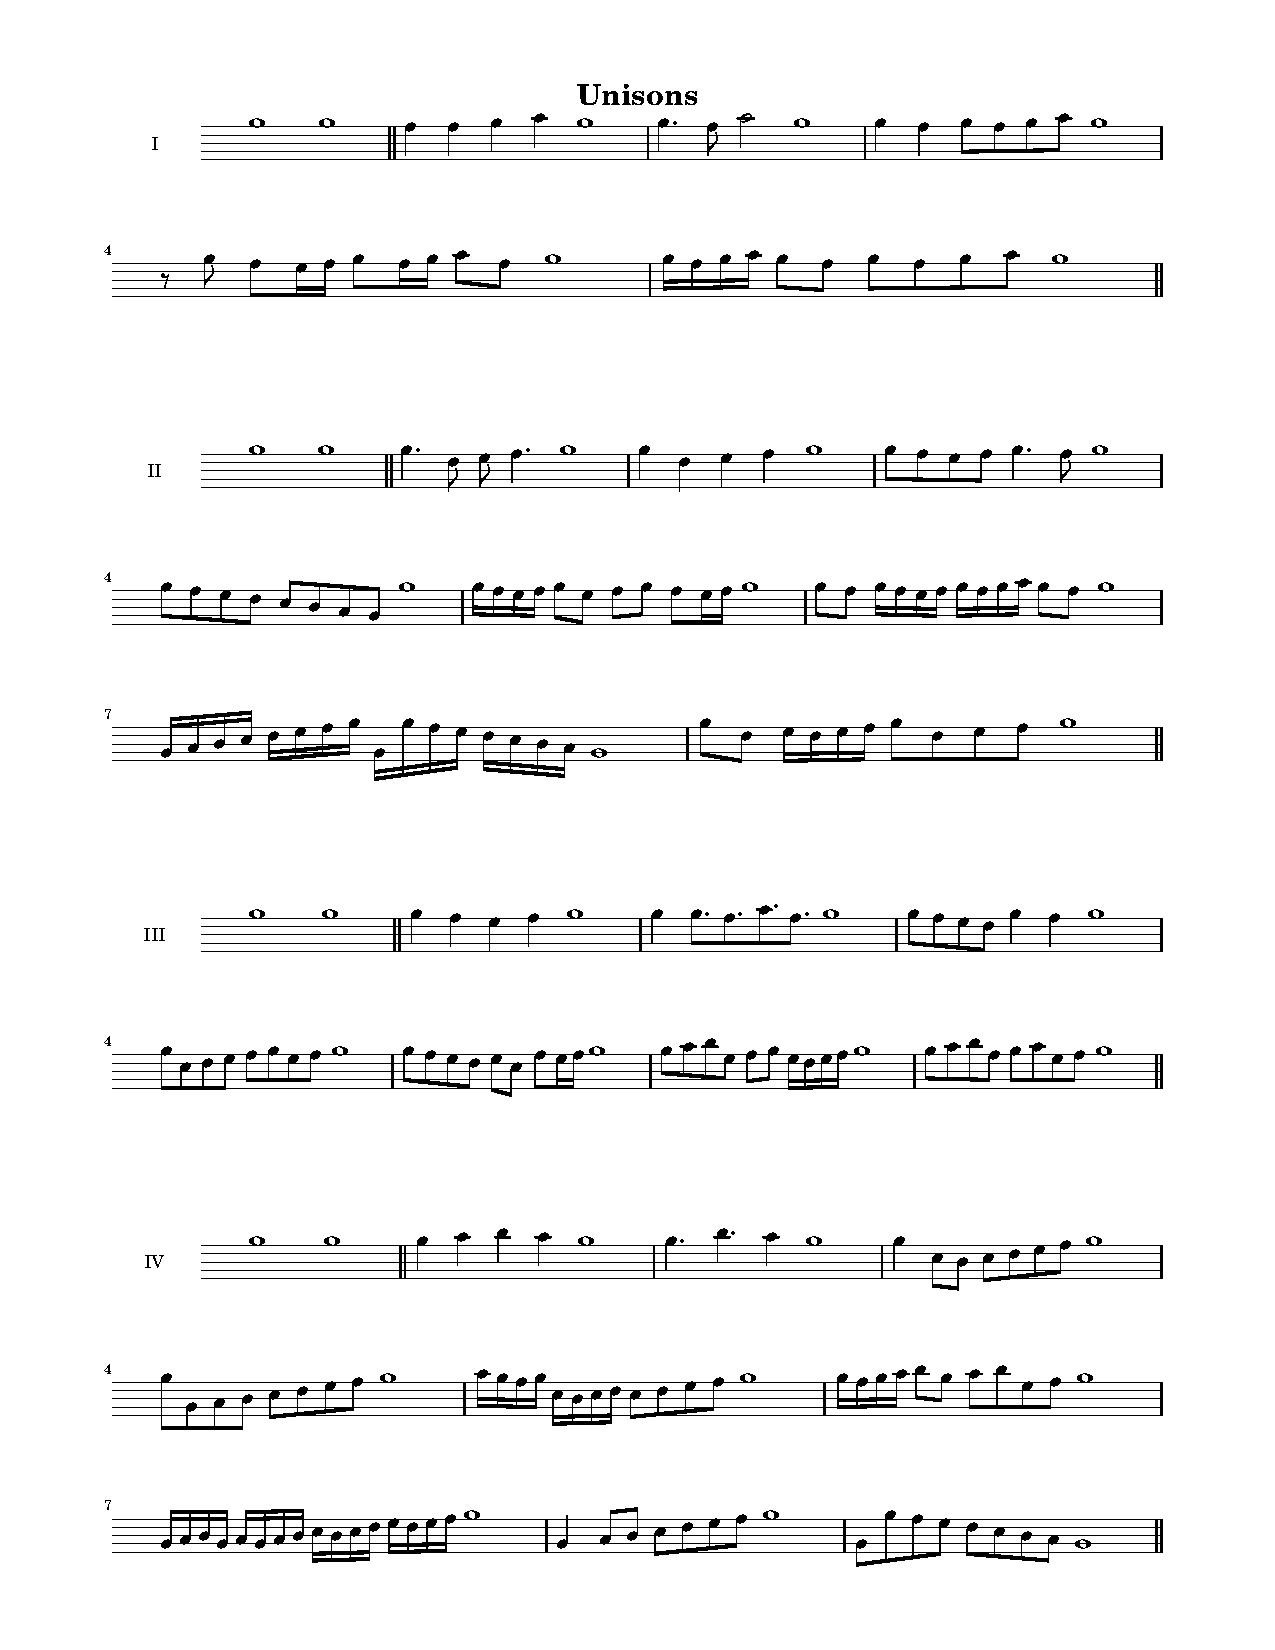
\includepdf[pages=-,pagecommand={},addtolist={1,figure,,unison},offset=0 -.12in,scale=0.97]{./unison.pdf}

\chaptermark{Ascending Second}\thispagestyle{FooBar}
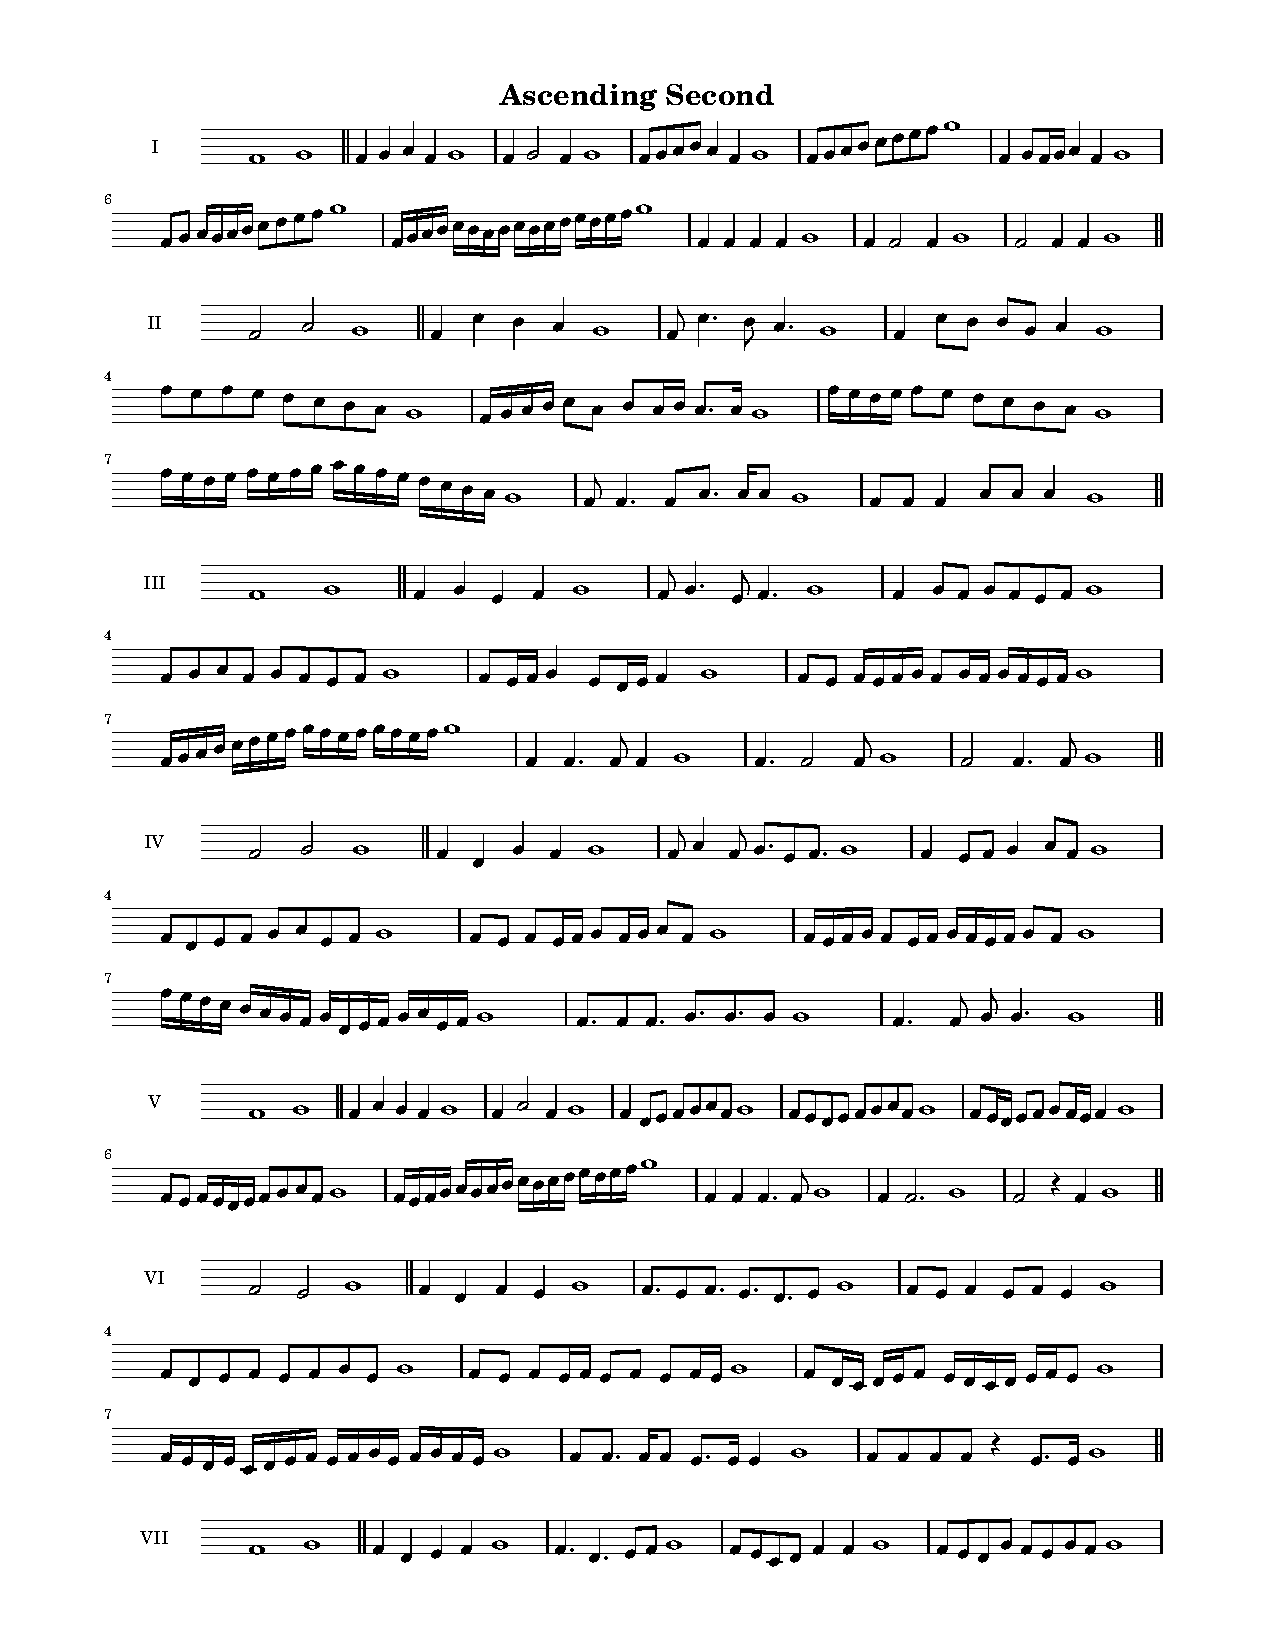
\includepdf[pages=-,pagecommand={},addtolist={1,figure,,ascending_second},offset=0 -.12in,scale=0.97]{./ascending_second.pdf}

\chaptermark{Descending Second}\thispagestyle{FooBar}
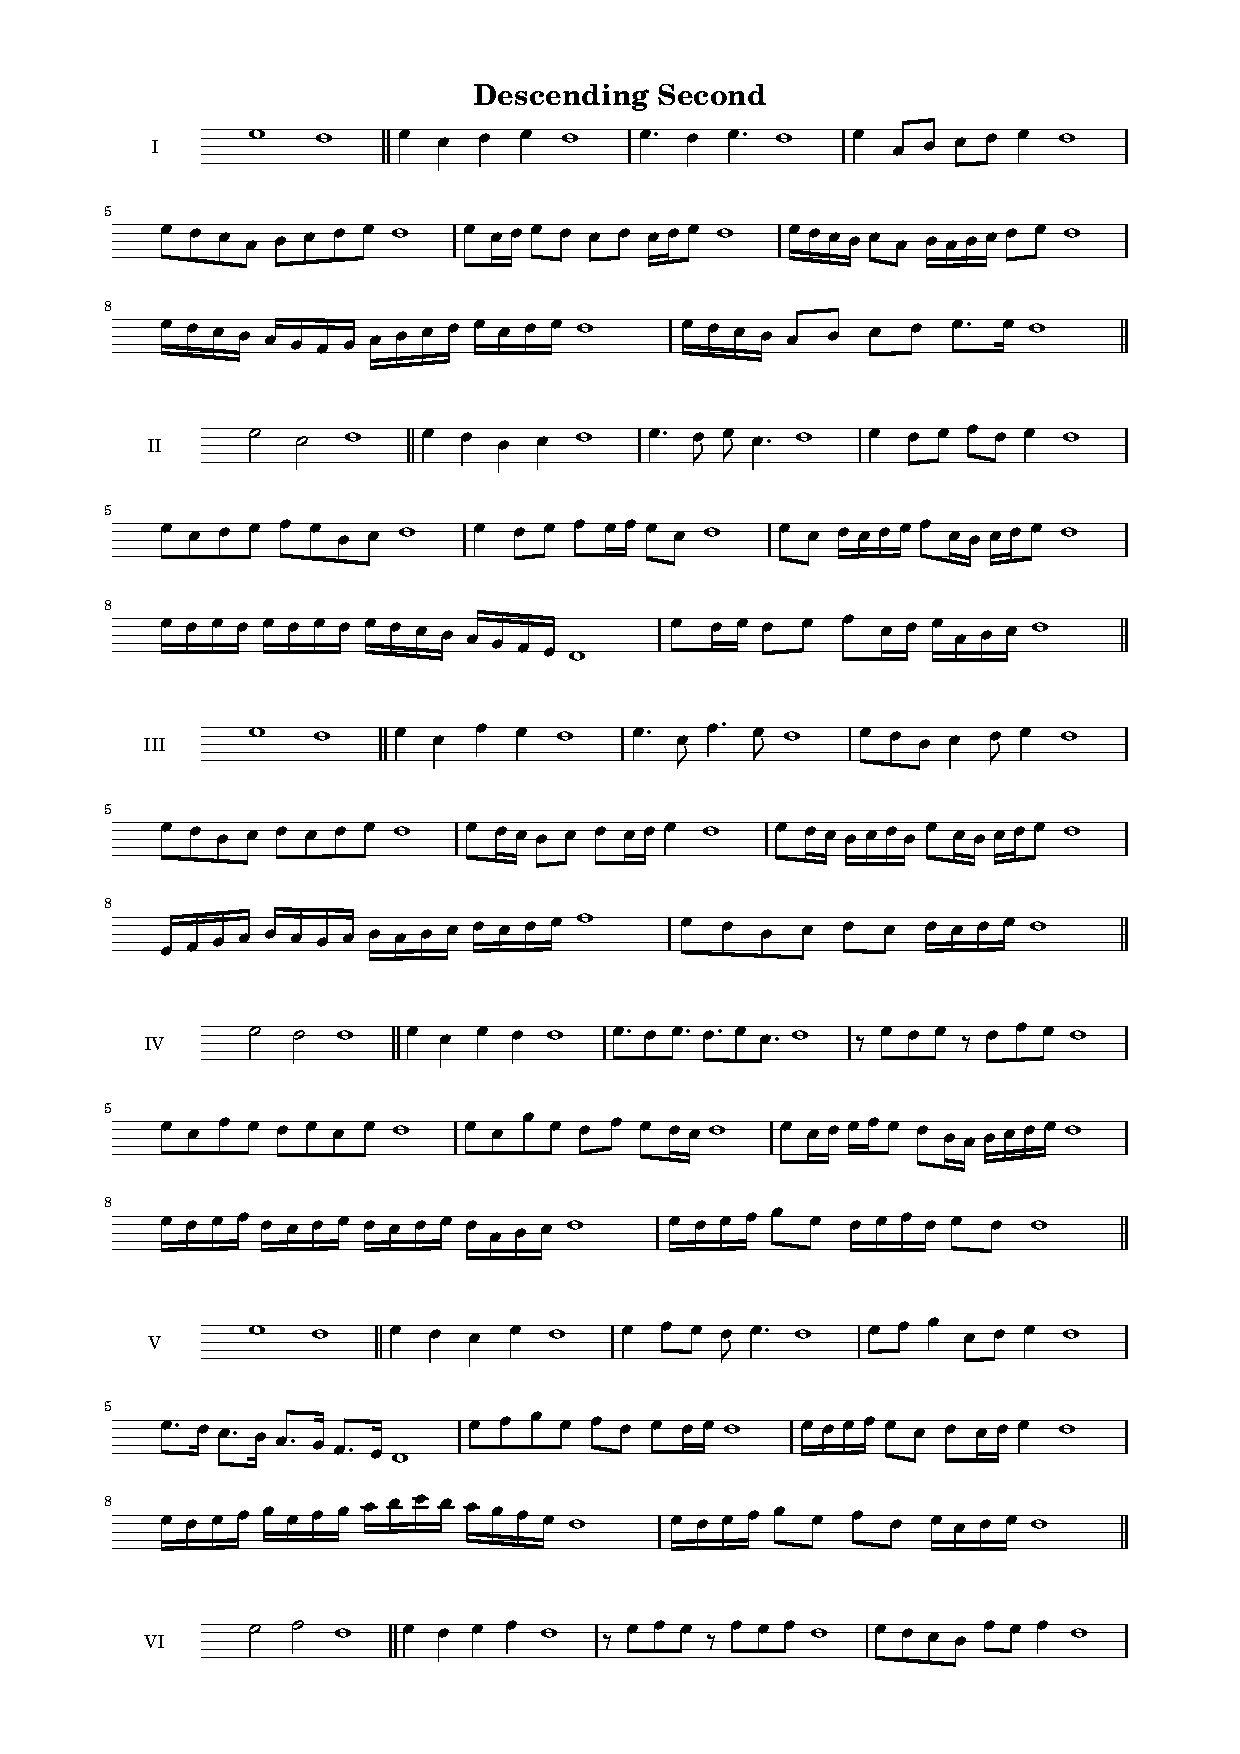
\includepdf[pages=-,pagecommand={},addtolist={1,figure,,descending_second},offset=0 -.12in,scale=0.97]{./descending_second.pdf}

\chaptermark{Ascending Third}\thispagestyle{FooBar}
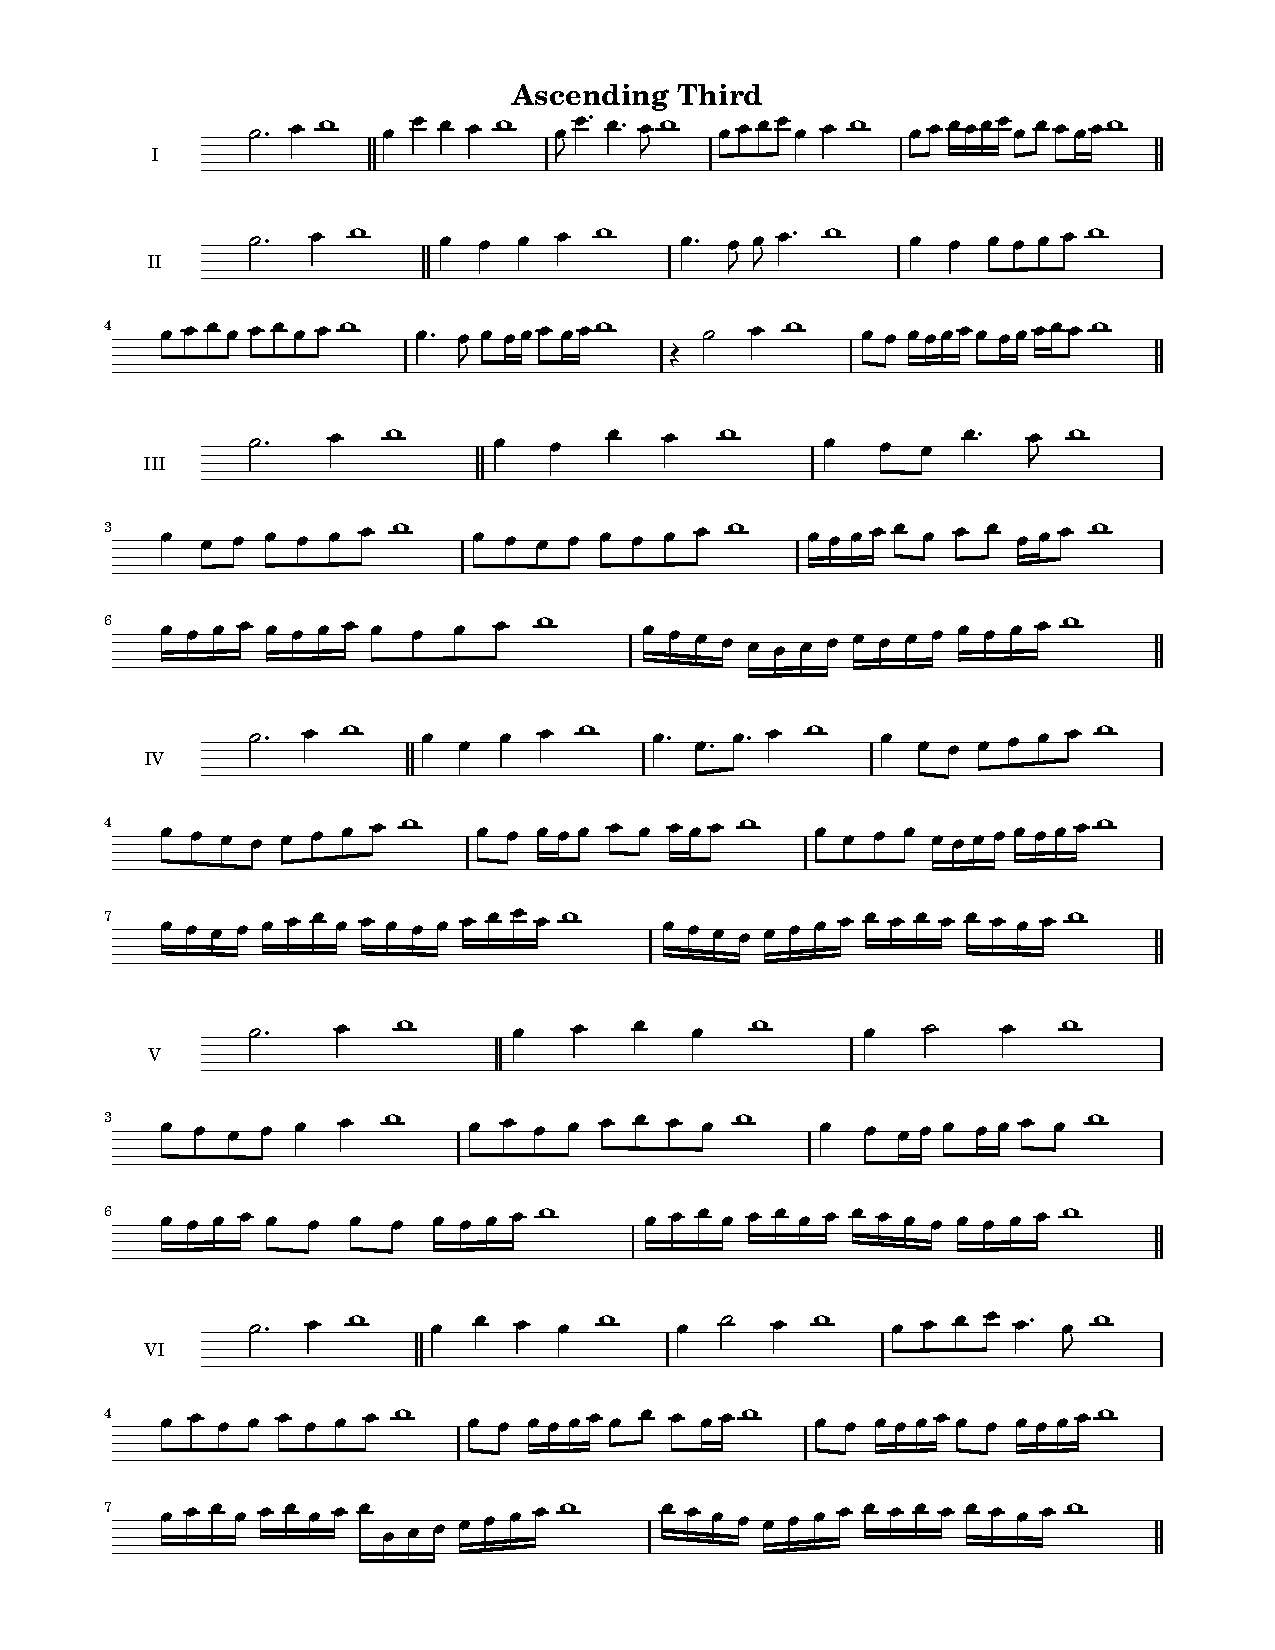
\includepdf[pages=-,pagecommand={},addtolist={1,figure,,ascending_third},offset=0 -.12in,scale=0.97]{./ascending_third.pdf}
\chaptermark{Descending Third}\thispagestyle{FooBar}
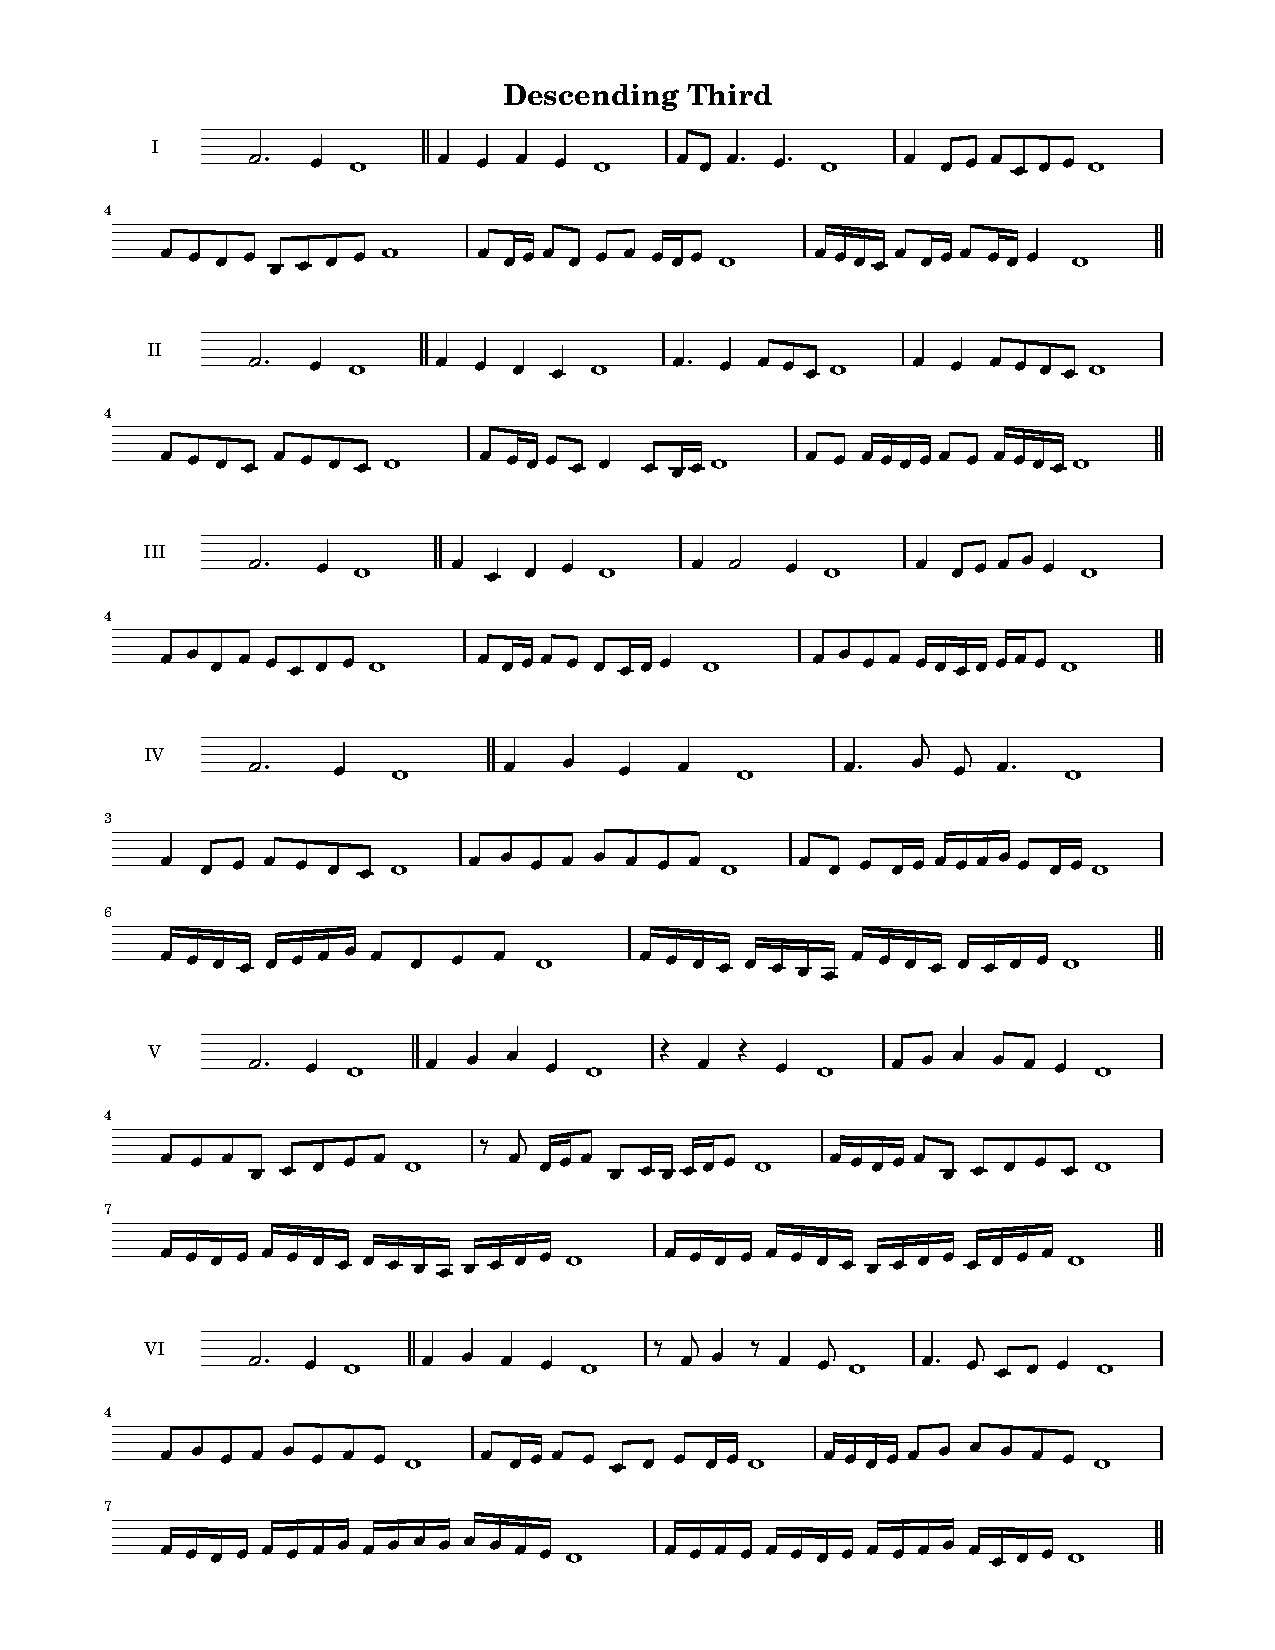
\includepdf[pages=-,pagecommand={},addtolist={1,figure,,descending_third},offset=0 -.12in,scale=0.97]{./descending_third.pdf}

\chaptermark{Ascending Fourth}\thispagestyle{FooBar}
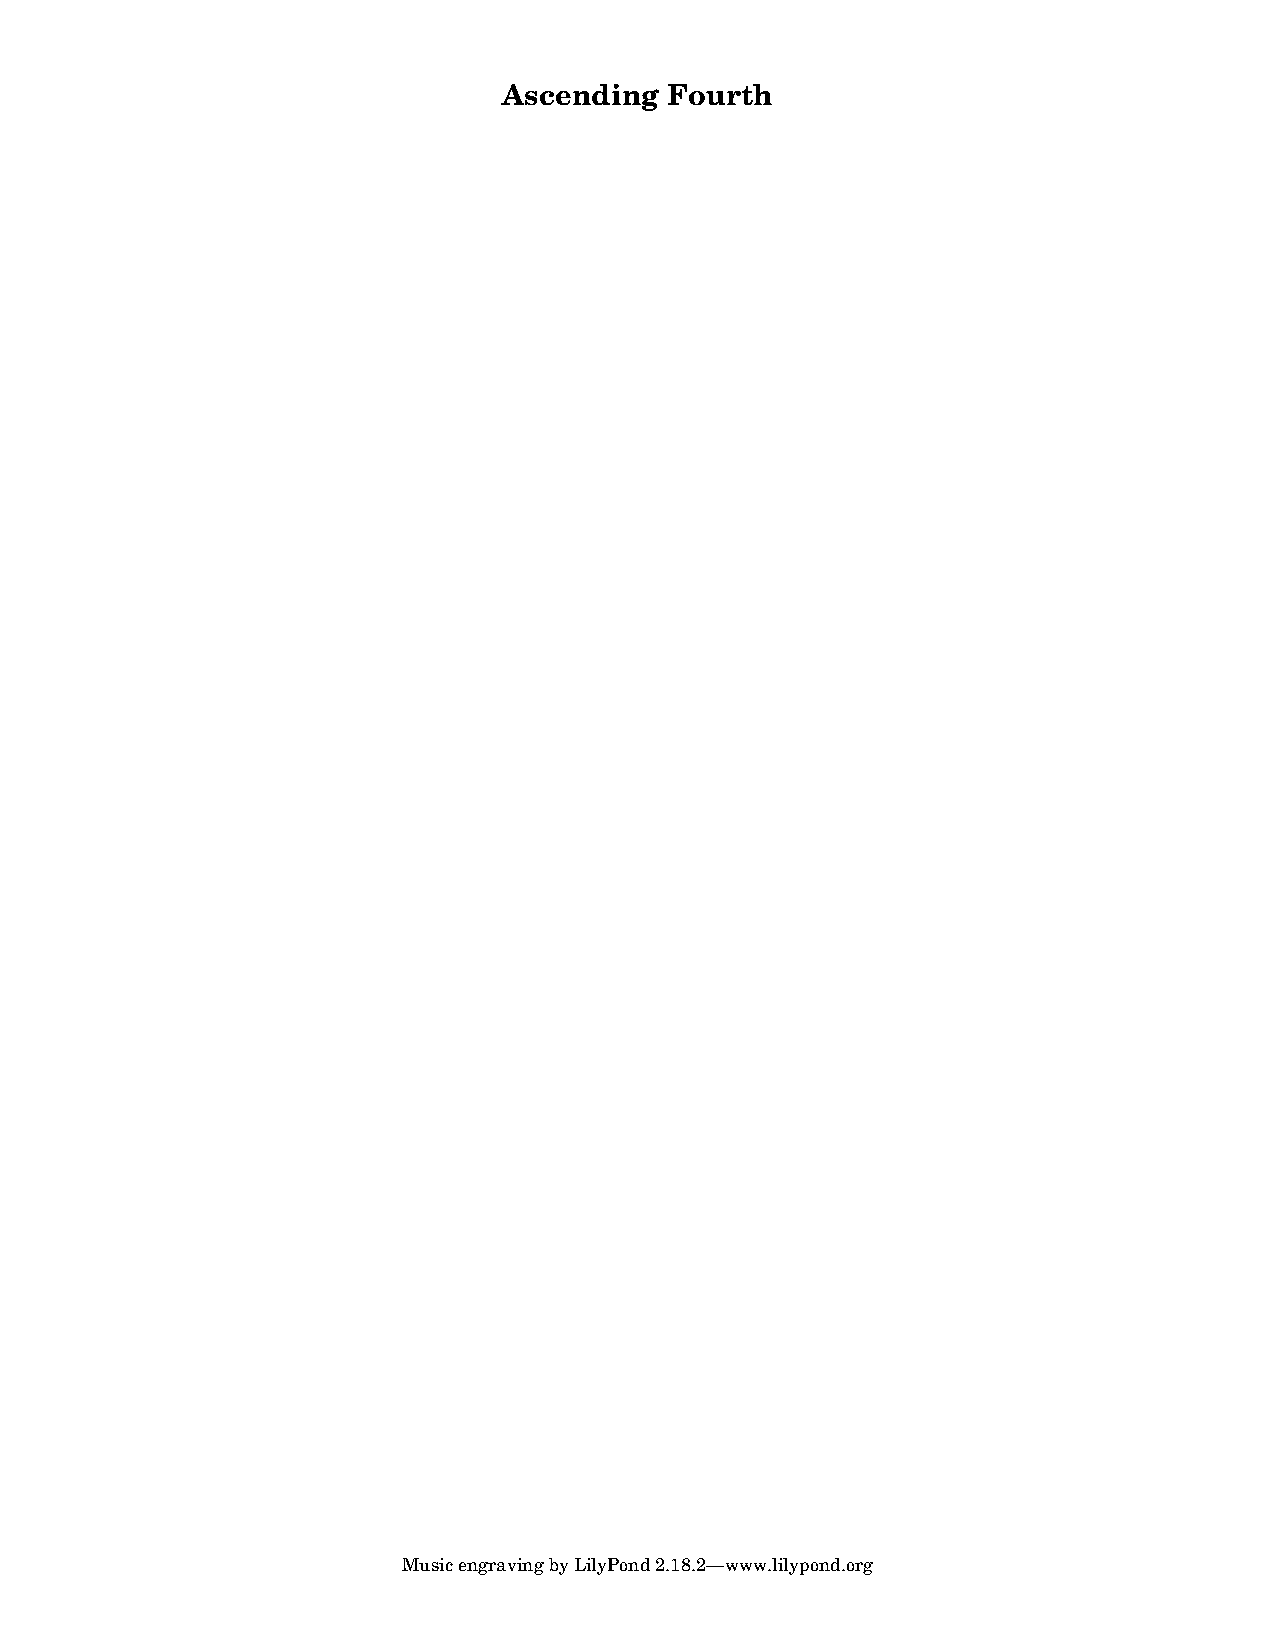
\includepdf[pages=-,pagecommand={},addtolist={1,figure,,ascending_fourth},offset=0 -.12in,scale=0.97]{./ascending_fourth.pdf}

\chaptermark{Descending Fourth}\thispagestyle{FooBar}
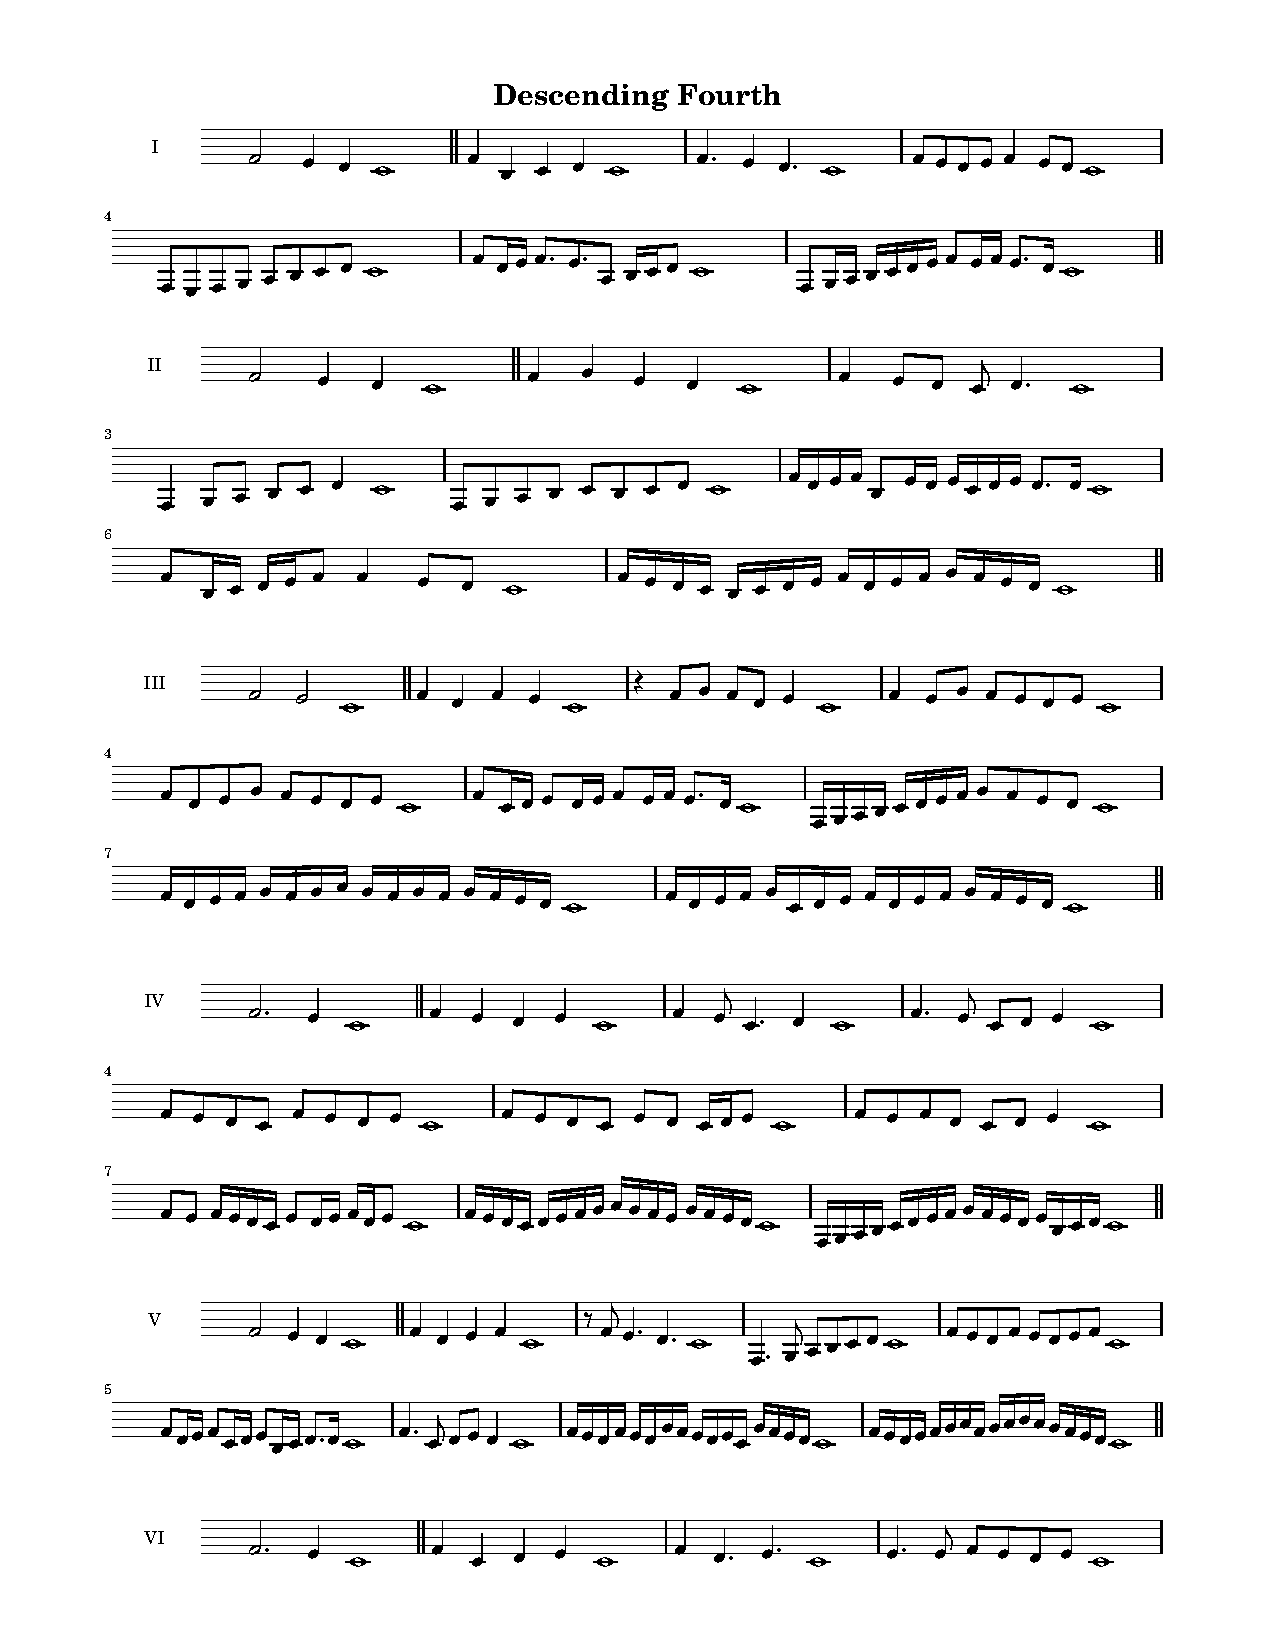
\includepdf[pages=-,pagecommand={},addtolist={1,figure,,descending_fourth},offset=0 -.12in,scale=0.97]{./descending_fourth.pdf}

\chaptermark{Ascending Fifth}\thispagestyle{FooBar}
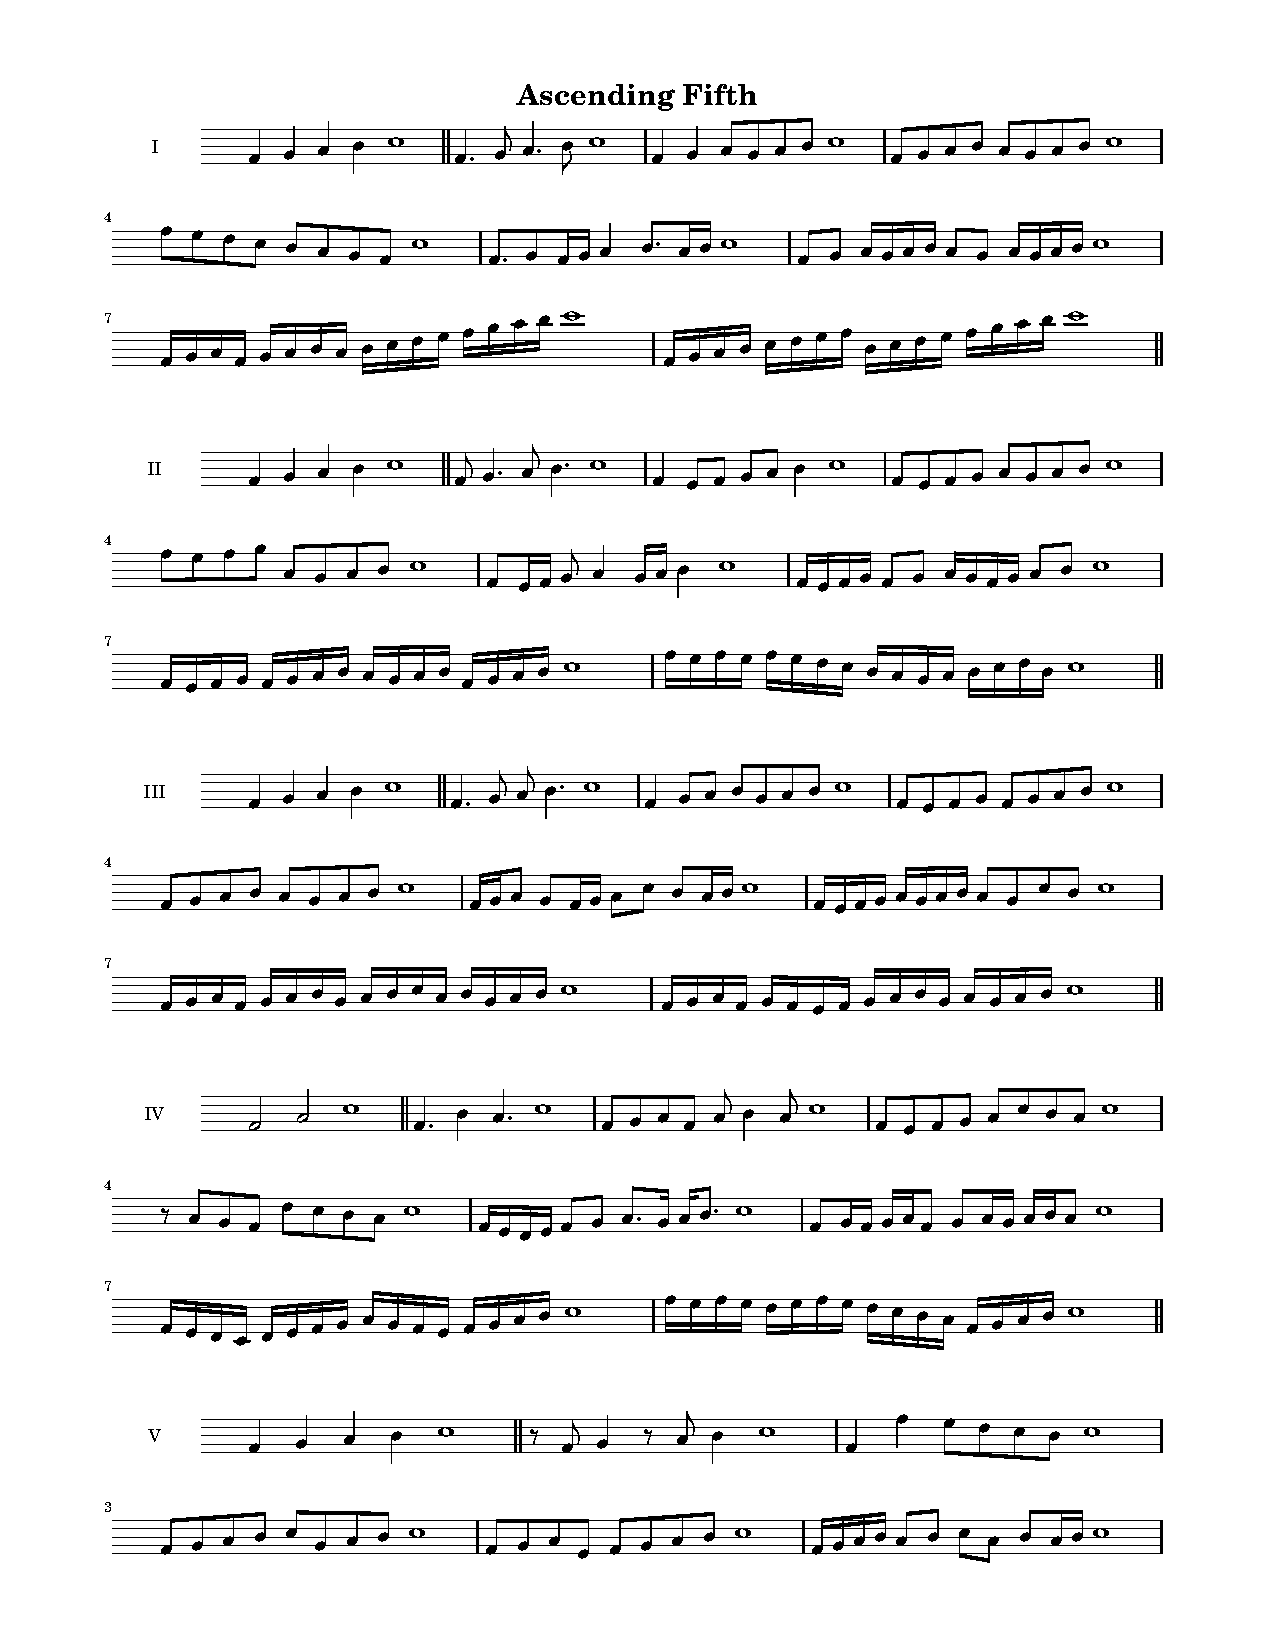
\includepdf[pages=-,pagecommand={},addtolist={1,figure,,ascending_fifth},offset=0 -.12in,scale=0.97]{./ascending_fifth.pdf}
\chaptermark{Descending Fifth}\thispagestyle{FooBar}
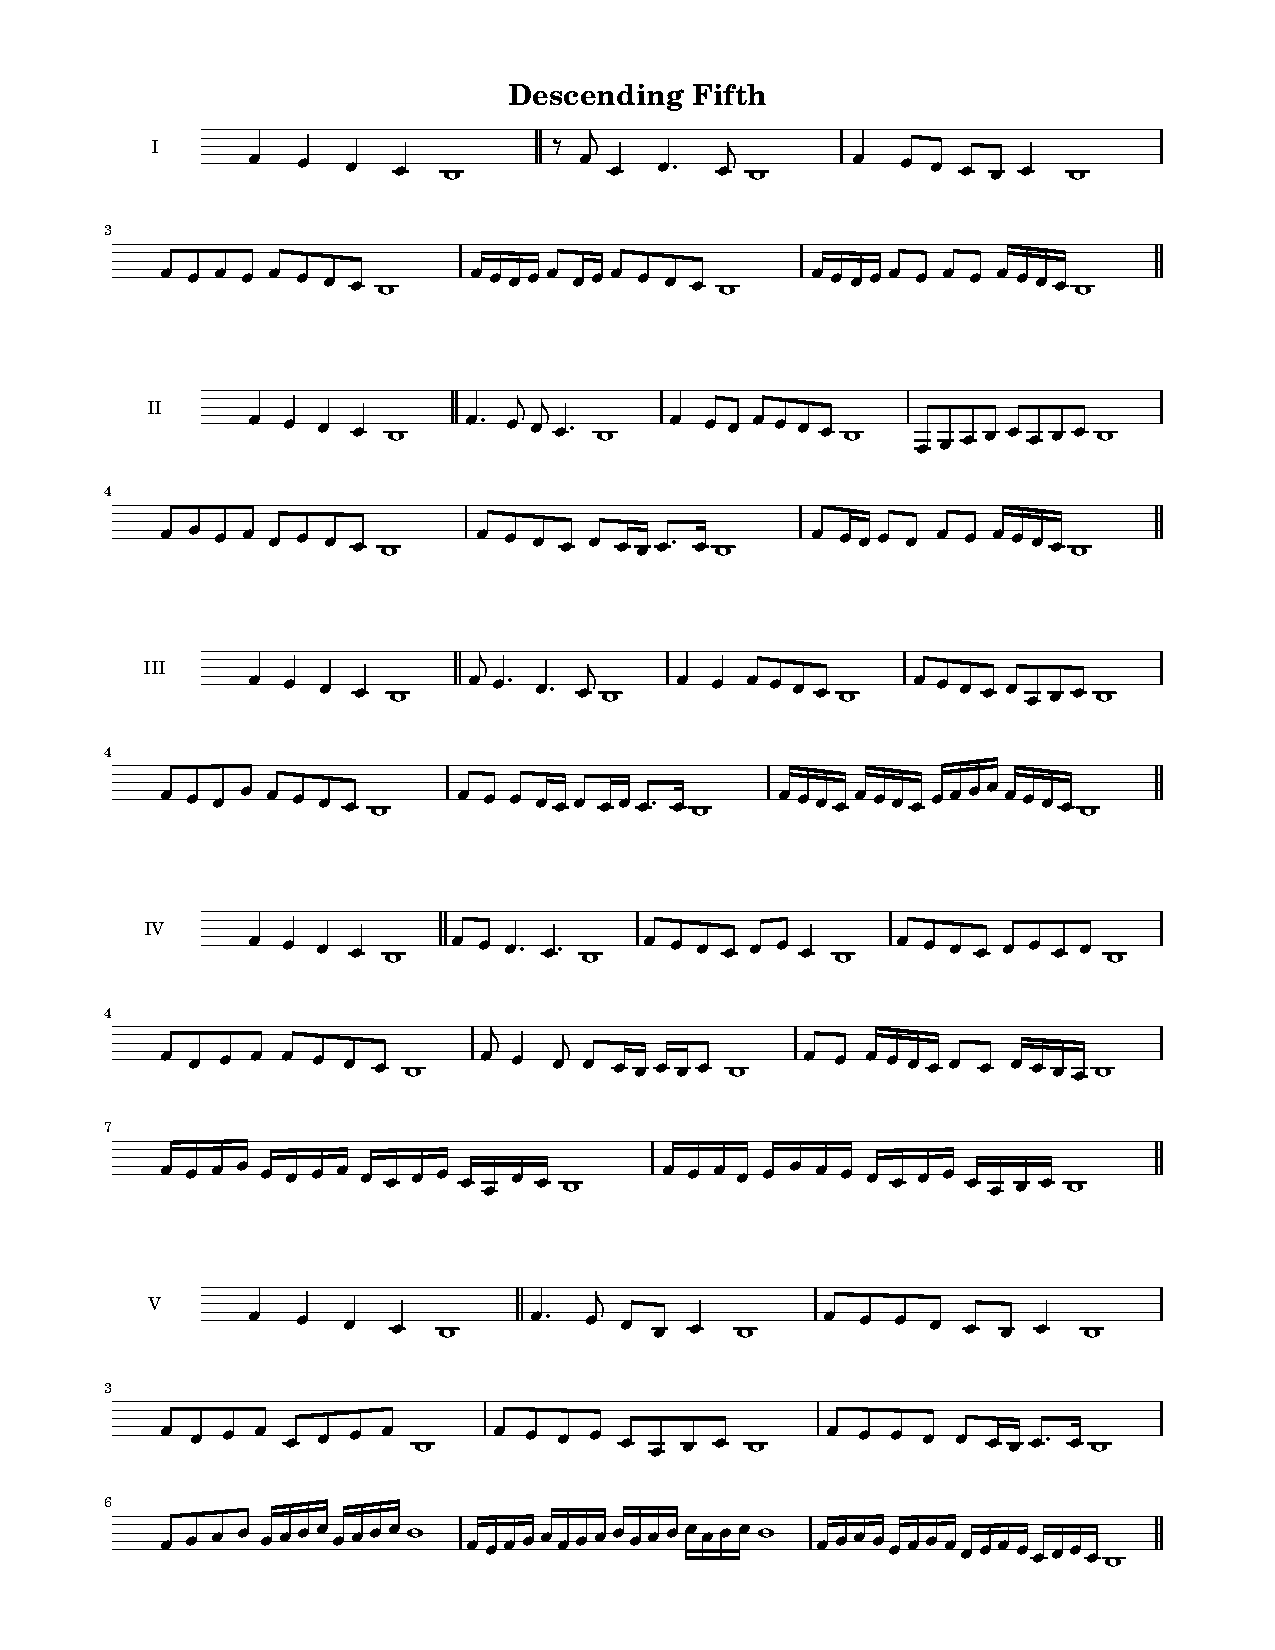
\includepdf[pages=-,pagecommand={},addtolist={1,figure,,descending_fifth},offset=0 -.12in,scale=0.97]{./descending_fifth.pdf}
\chaptermark{Cadences}\thispagestyle{FooBar}
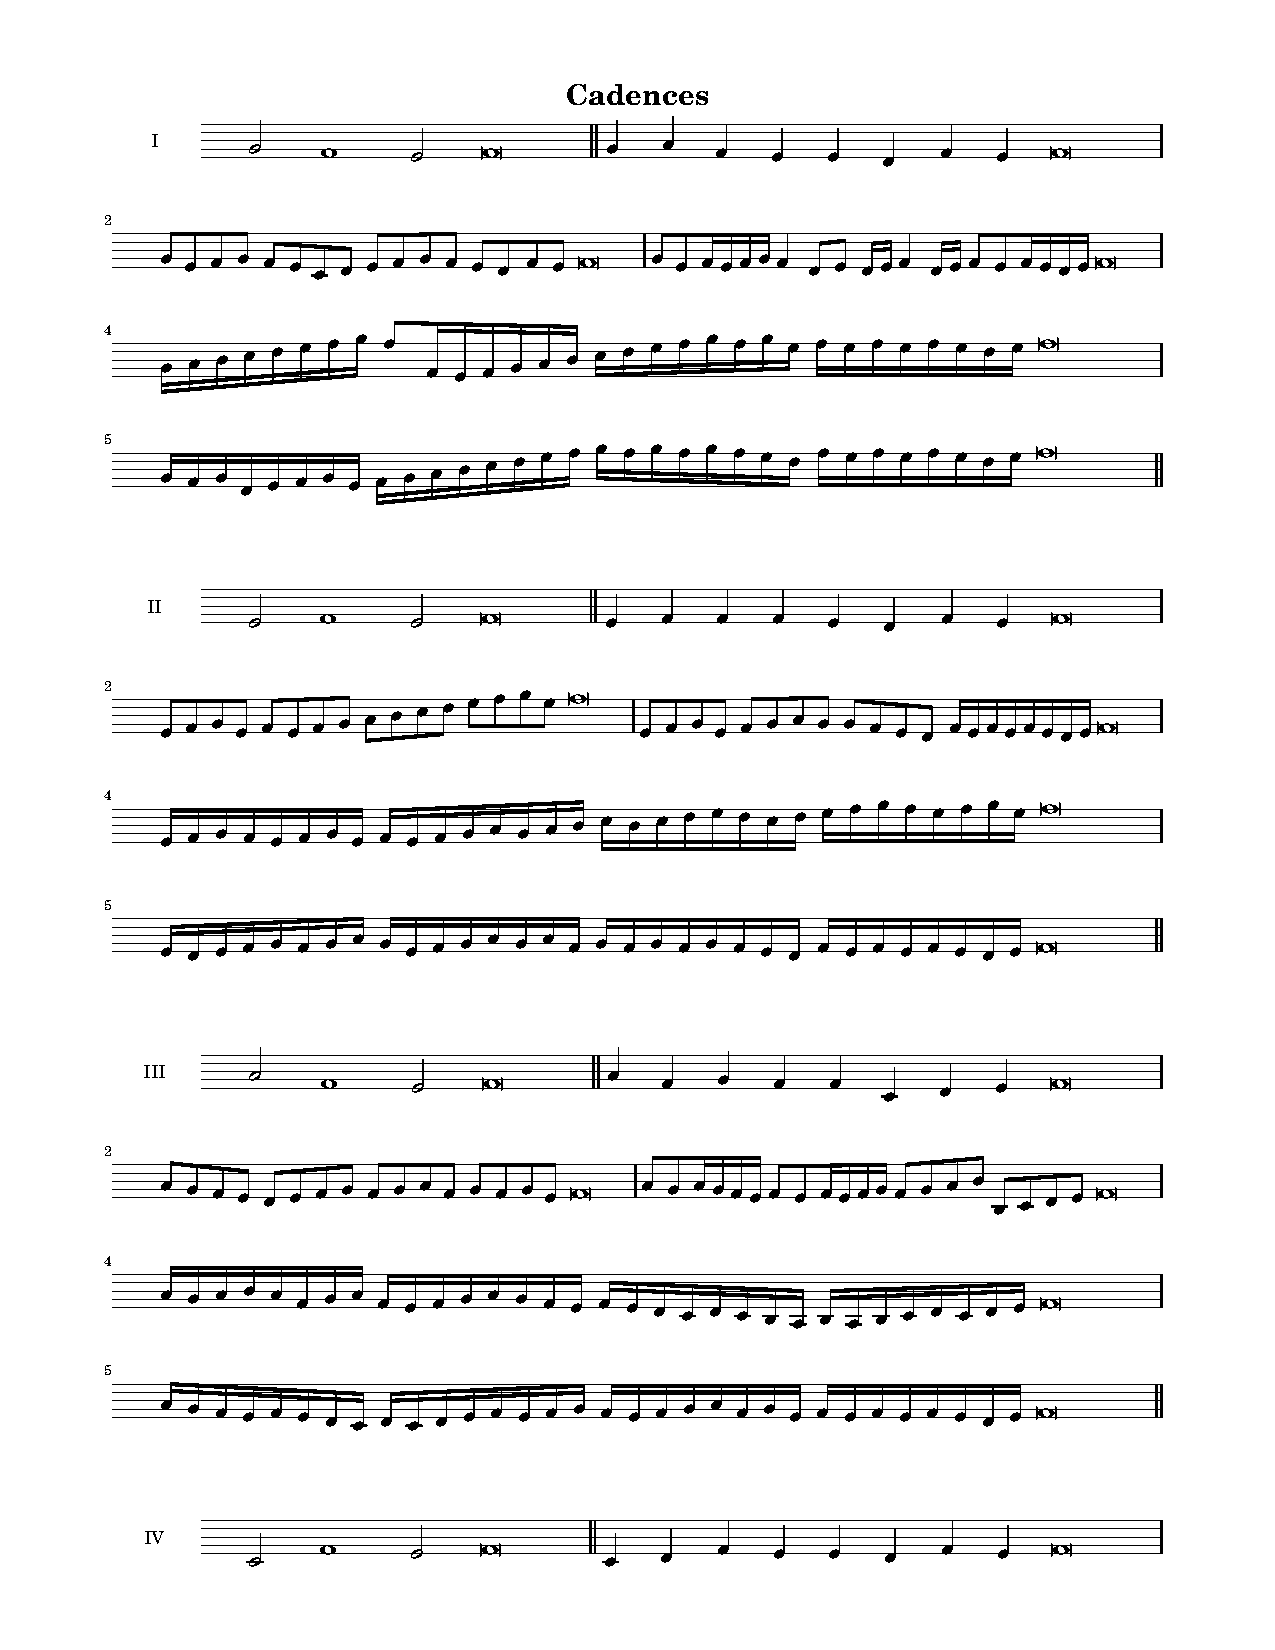
\includepdf[pages=-,pagecommand={},addtolist={1,figure,,cadences},offset=0 -.12in,scale=0.97]{./cadences.pdf}
\end{document}
